%% LyX 2.0.2 created this file.  For more info, see http://www.lyx.org/.
%% Do not edit unless you really know what you are doing.
\documentclass[english]{article}
\usepackage[T1]{fontenc}
\usepackage[latin9]{inputenc}
\usepackage{float}
\usepackage{graphicx}
\usepackage{babel}
\begin{document}
\begin{figure}[H]
\begin{centering}
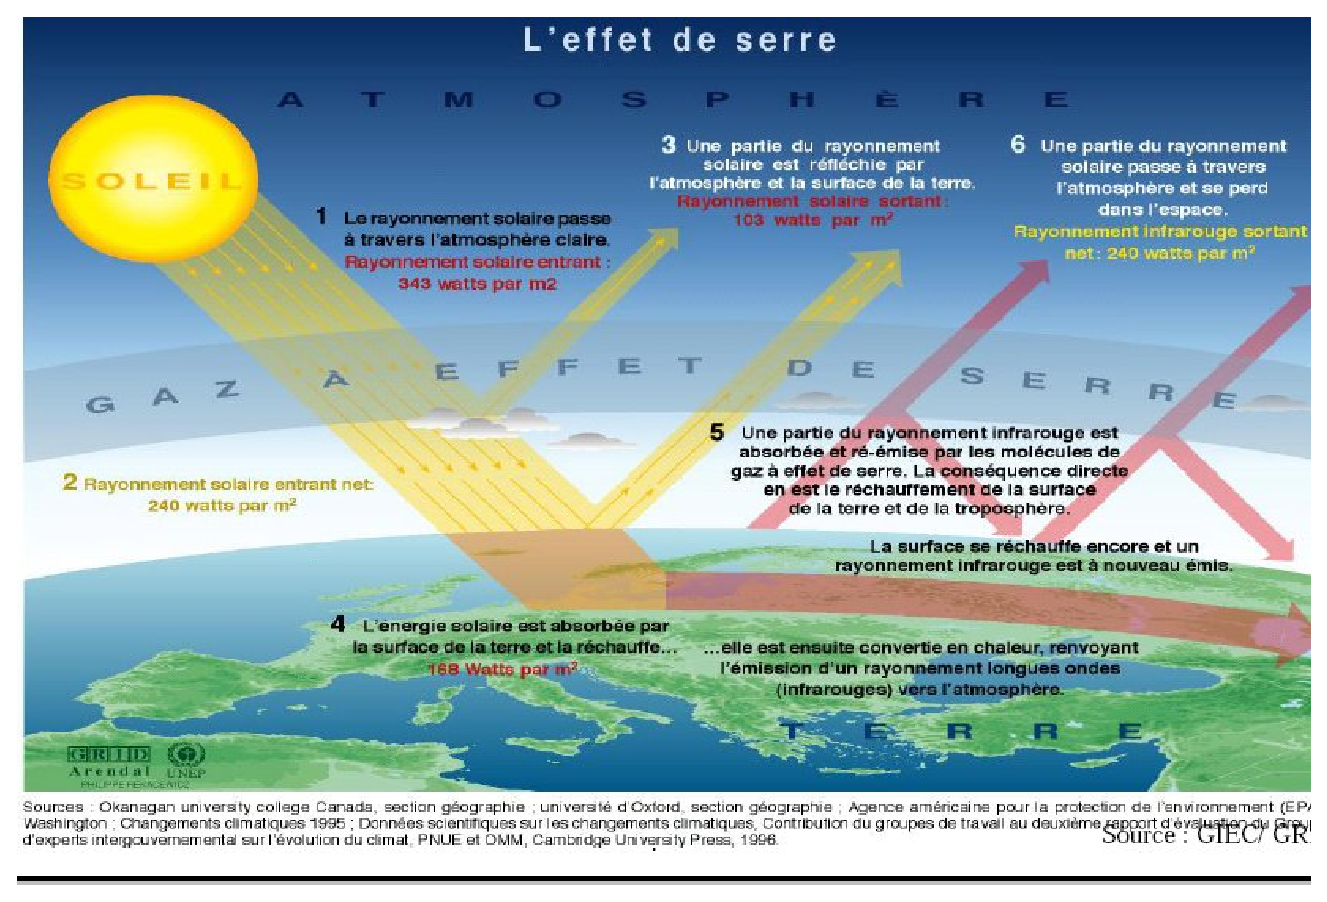
\includegraphics[angle=90]{effet-serre}
\par\end{centering}

\caption{scq}


\end{figure}


\begin{figure}[H]
\begin{centering}
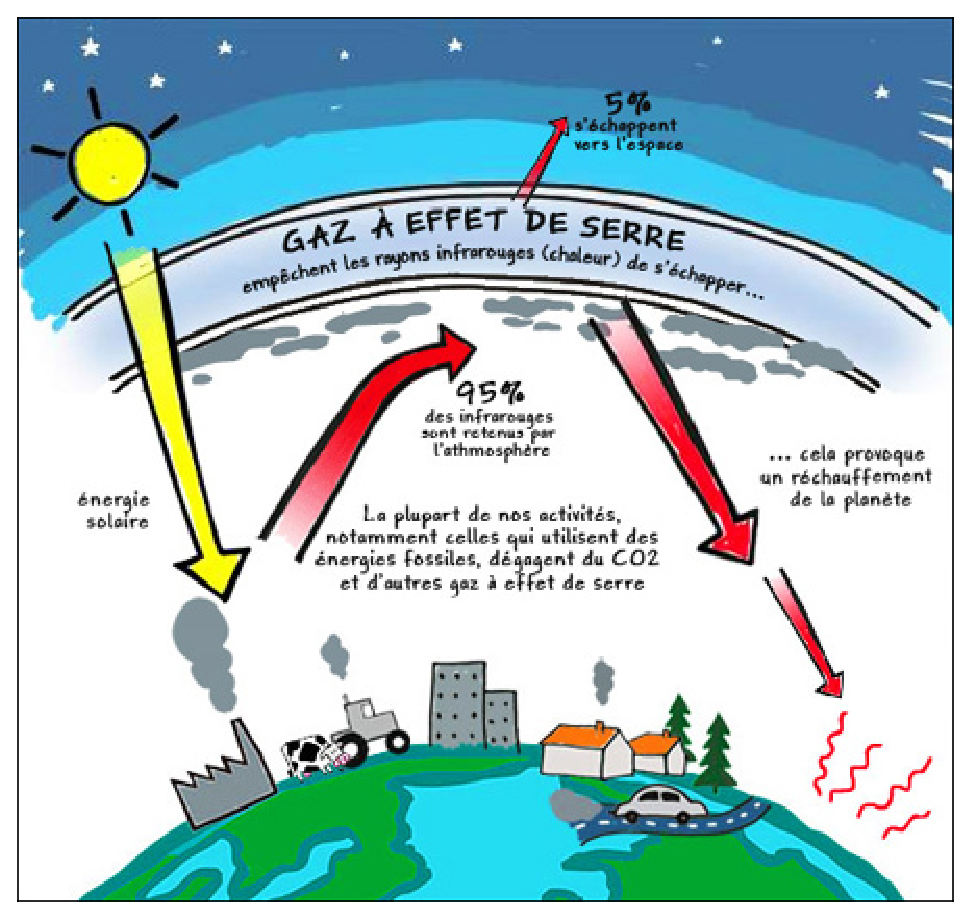
\includegraphics[scale=0.8]{effet_serre2}
\par\end{centering}

\caption{scq}
\end{figure}


\begin{figure}[H]
\begin{centering}
\includegraphics[scale=0.8]{effet-de-serre}
\par\end{centering}

\caption{scq}
\end{figure}


\begin{figure}[H]
\begin{centering}
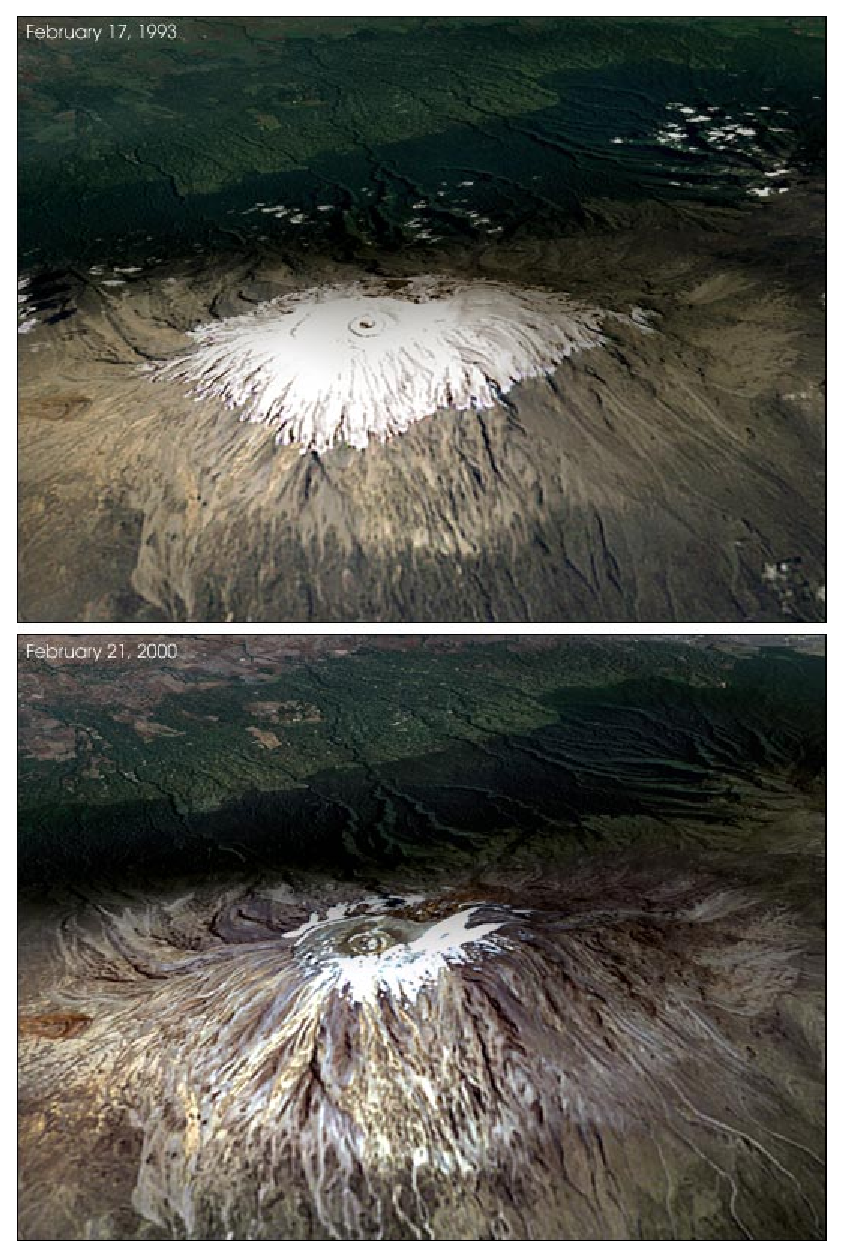
\includegraphics[scale=0.8]{kili}
\par\end{centering}

\caption{scq}
\end{figure}


\begin{figure}[H]
\begin{centering}
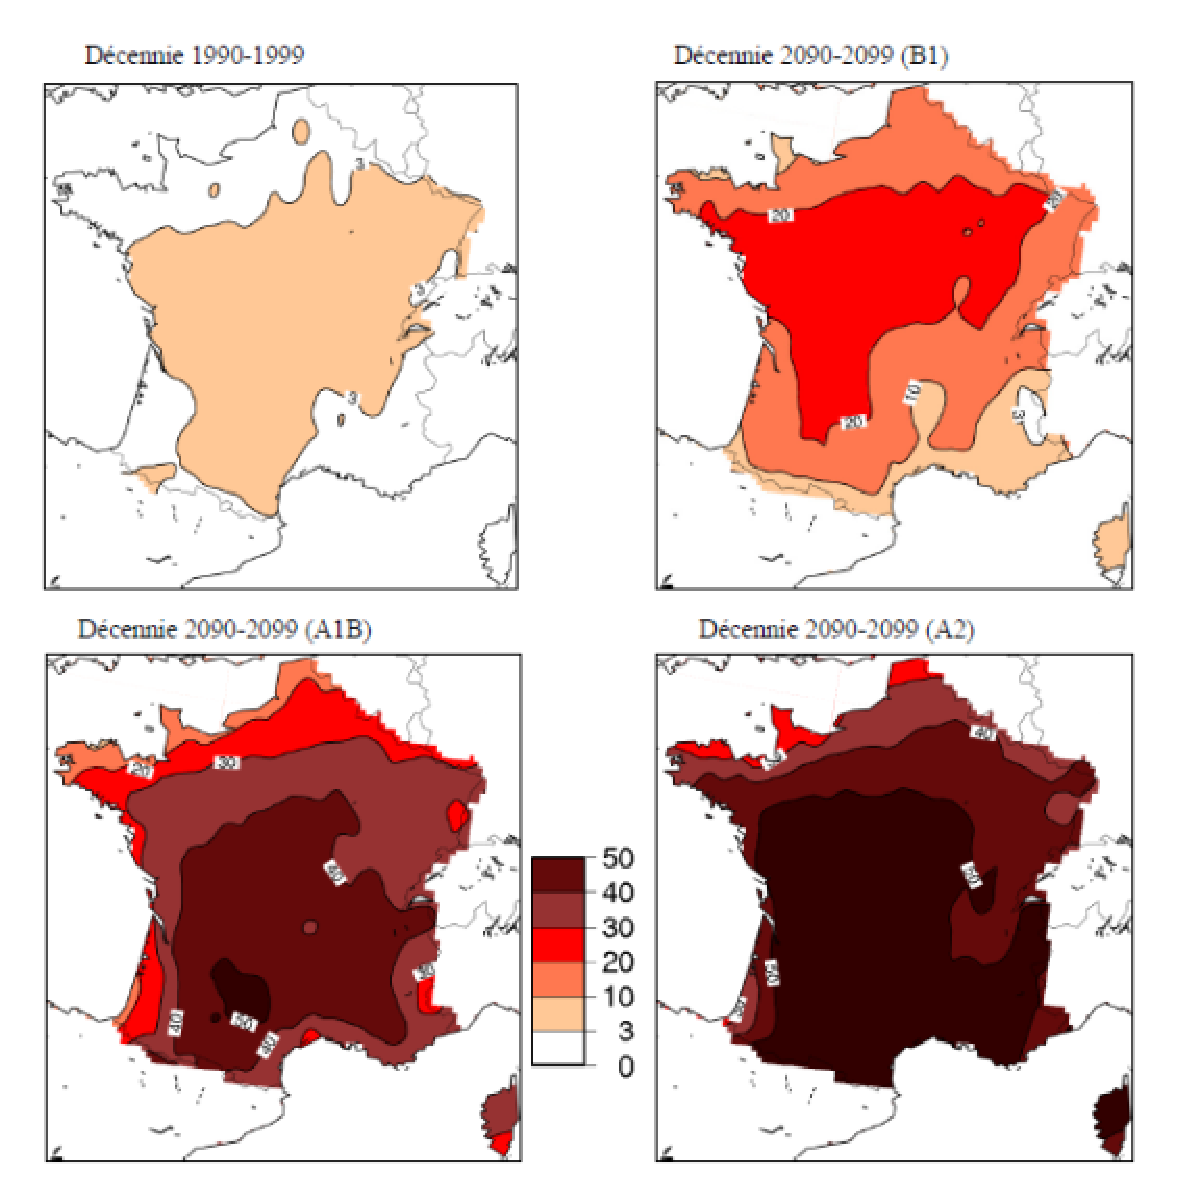
\includegraphics[scale=0.8]{35france}
\par\end{centering}

\caption{scq}
\end{figure}


\begin{figure}[H]
\begin{centering}
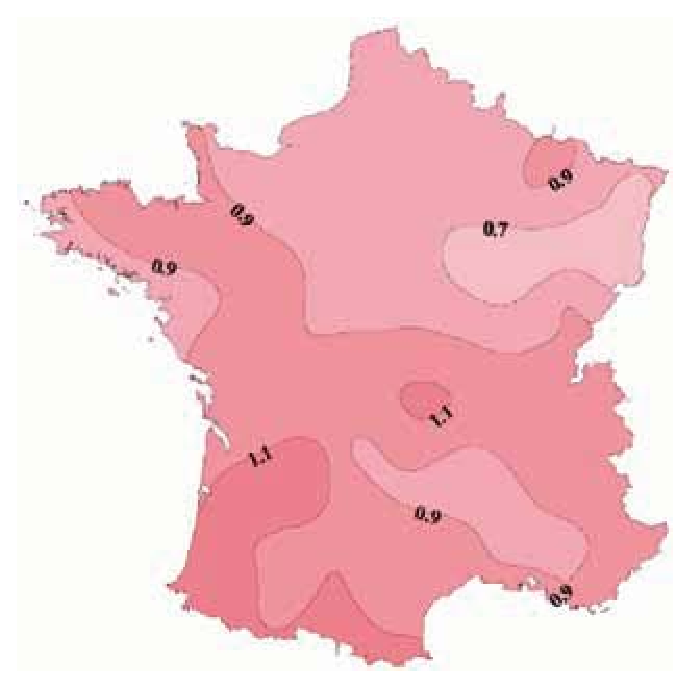
\includegraphics[scale=0.8]{franceMoyenne}
\par\end{centering}

\caption{scq}
\end{figure}

\end{document}
